\section{Квазистационарные электромагнитные поля. Уравнение диффузии для
магнитного поля. Скин-эффект.}

\subsection*{Скин-эффект}

\begin{minipage}[c]{0.4\textwidth} % Левая часть: изображение
    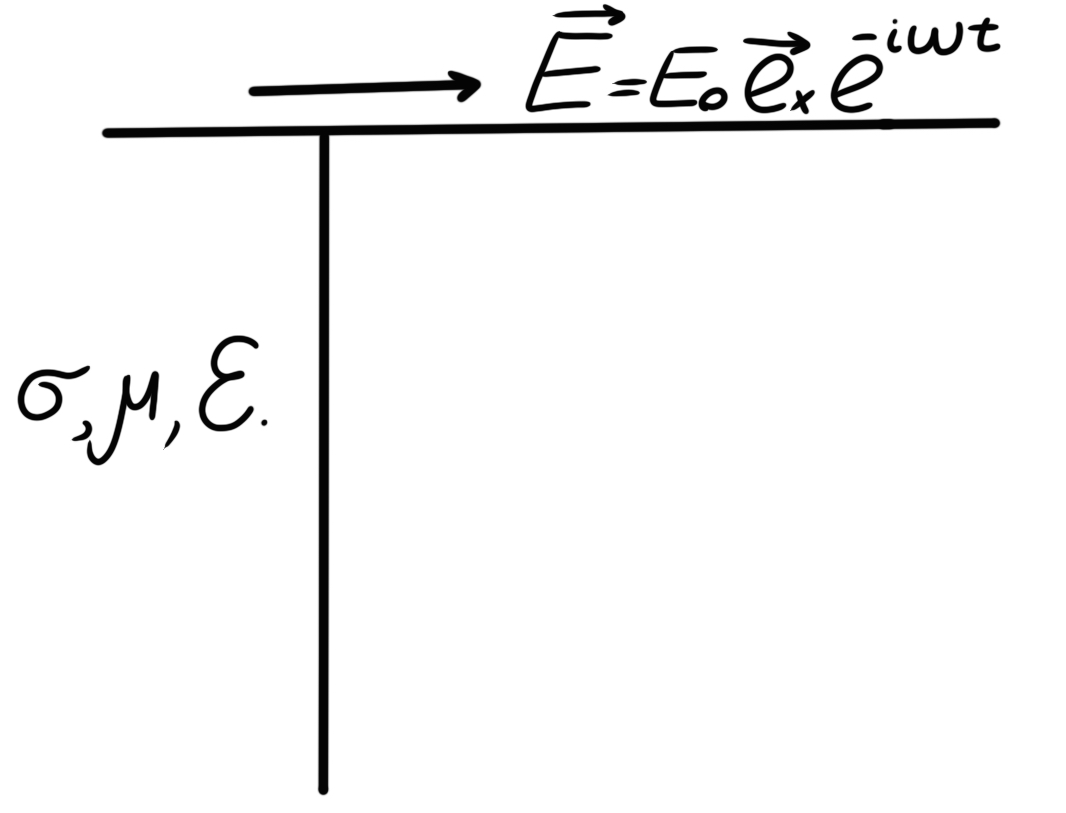
\includegraphics[width=\textwidth]{im/90.png}% Ваше изображение
\end{minipage}%
\hfill
\begin{minipage}[c]{0.6\textwidth} % Правая часть: текст
   \[
    \begin{cases}
        \mathrm{div}\vec{E}=0 \\
         \mathrm{rot}\vec{E}=-\frac{1}{c}\frac{\partial \vec{B}}{\partial t}=-\frac{\mu}{c} \frac{\partial \vec{H}}{\partial t} \\
         \mathrm{div}\vec{B}=0 \\
         \mathrm{rot}\vec{H}=\frac{4\pi}{c}\sigma\vec{E}+\cancelto{0}{\frac{1}{c}\frac{\partial\varepsilon\vec{E}}{\partial t}  }(\text{при малых частотах принебрег.})   
    \end{cases}
    \]
    Последним членом можно принебречь при малых частотах, если \( \frac{\sigma E}{c}>>\varepsilon\omega E  \) \dots
\end{minipage}

\begin{gather*}
    \mathrm{rot}\mathrm{rot}\vec{E}=\cancelto{0}{\mathrm{grad}\mathrm{div}\vec{E} }-\Delta\vec{E} =-\frac{\mu}{c}\frac{\partial}{\partial t}\mathrm{rot}\vec{H}=-\frac{4\pi\mu\sigma}{c^2} \frac{\partial\vec{E}}{\partial t}\Rightarrow \\
    \Rightarrow \Delta\vec{E}=\frac {4\pi\mu\sigma} {c^2} \frac{\partial \vec{E}}{\partial t} 
\end{gather*}

Ищем решение в виде : \( \vec{E}=E_0\vec{e}_x e^{-i\omega t}e^{ikt}   \)

\[
\Delta\vec{E}=\frac{\partial^2 \vec{E}}{\partial z^2} =\frac{\partial}{\partial z} (ik\vec{E})=-k^2 \vec{E}
\]

\begin{gather*}
    \frac{\partial\vec{E}}{\partial t}=-i\omega\vec{E} \\
    -k^2\vec{E}=-\frac{4\pi i\omega\mu\sigma}{c^2}\vec{E}\Rightarrow k=\sqrt{i} \frac{\sqrt{4\pi\mu\sigma\omega}}{c} =\frac{\sqrt{2\pi\mu\sigma\omega}}{c}(1+i)=: \frac{1+i}{\delta}  \\
    \boxed{\delta:=\frac{c}{\sqrt{2\pi\mu\sigma\omega}} }-\textit{толщина скин слоя} \\
    \vec{E}=E_0\vec{e}_x e^{i\left( \frac{z}{\delta}-\omega t \right) }e^{-\frac{z}{\delta} }  
\end{gather*}

\imc[0.8\textwidth]{91.png}

\[
e^{-\pi}=\frac{1}{e^{\pi} }\backsim 0,1 
\]

(1)-область где Е заметно отличимо от нуля над скин слоем.

Скин эффект считается сильным если \( \delta \)- мало и наоборот.

\subsection*{Уравнение диффузии для
магнитного поля}

\[
\vec{j}_n\overset{df}{=}=D\grad n \qquad \frac{\partial n}{\partial t} =\mathrm{div}\vec{j}_n=0 
\]

\begin{minipage}[c]{0.2\textwidth} % Левая часть: изображение
    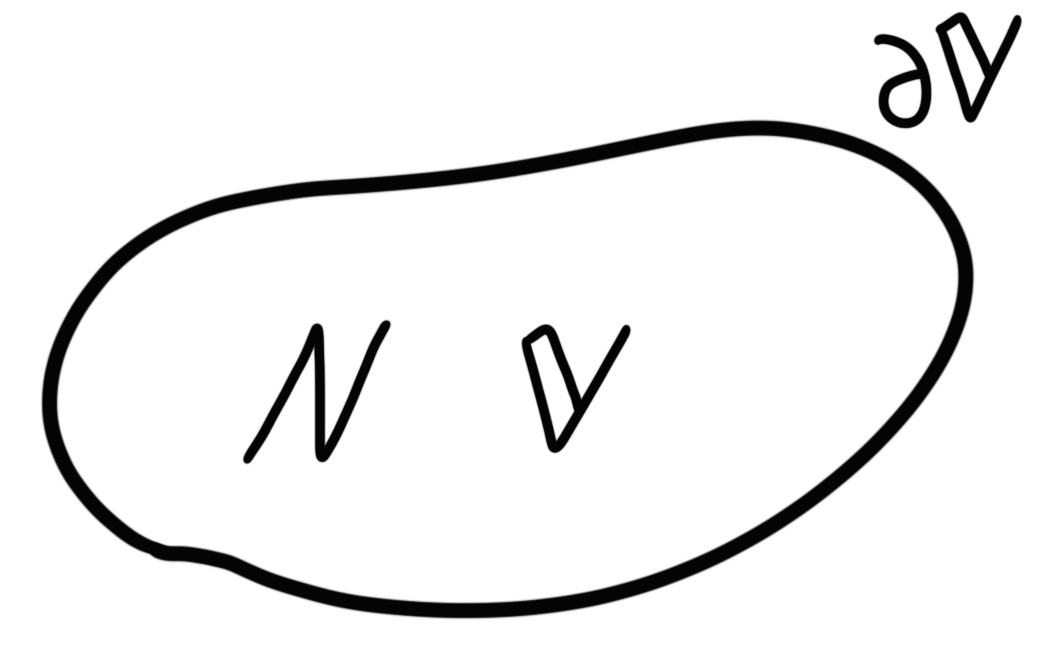
\includegraphics[width=\textwidth]{im/92.png}% Ваше изображение
\end{minipage}%
\hfill
\begin{minipage}[c]{0.6\textwidth} % Правая часть: текст
   \[
   \frac{dN}{dt}=\oiint \vec{j}_nd\vec{S}
   \]
\end{minipage}

\begin{gather*}
    \underset{\mathbb{V}}{\iiint} \frac{\partial n}{\partial t} dV=-\underset{\mathbb{V}}{\iiint}\mathrm{div}\vec{j}_n \, dV \Rightarrow \frac{\partial n}{\partial t}+\mathrm{div}\vec{j}_n=0, \\
    \frac{\partial n}{\partial t} + \nabla \cdot (-D \nabla n) = 0 \Rightarrow \boxed{\frac{\partial n}{\partial t} = D \Delta n}.
\end{gather*}